\documentclass[12pt,a4paper]{report}
%\documentclass[17pt]{extreport}
\usepackage[latin1]{inputenc}
\usepackage{ngerman}
\usepackage{makeidx,longtable,geometry,fancyhdr,color}
\usepackage{colortbl}
\usepackage[]{graphicx}
%-- dadurch werden zweizeilige Fussnoten einger�ckt
\usepackage[hang]{footmisc}
%-- refpage und bei dem Abk�rzungsverzeichniss steht die Seite auf der die Abk�rzung definiert wird
\usepackage[german,refpage]{nomencl}



\usepackage{enumitem}
\setlist{noitemsep,topsep=0.5cm}

\definecolor{dunkelgrau}{gray}{0.55}
\definecolor{hellgrau}{gray}{0.90}

\usepackage{listings}
\lstset{basicstyle=\footnotesize, numbers=left, numberstyle=\tiny, stepnumber=1,numbersep=10pt, firstnumber=1, backgroundcolor=\color{hellgrau}, frame=shadowbox, rulesepcolor=\color{dunkelgrau},
framesep=5pt, framerule=0.75pt, captionpos=b, breaklines=true, breakatwhitespace=false, escapeinside={!*}{*!},
aboveskip=0.25cm}

\renewcommand{\lstlistlistingname}{Quellcode Verzeichnis}
\renewcommand{\lstlistingname}{Quellcode}


% variable referenzennamen
\usepackage[german]{varioref}
\labelformat{lstlisting}{Quellcode~#1}
\labelformat{chapter}{Kapitel~#1}
\labelformat{section}{Abschnitt~#1}
\labelformat{subsection}{Unterabschnitt~#1}
\labelformat{subsubsection}{Unterunterabschnitt~#1}
\labelformat{paragraph}{Absatz~#1}
\labelformat{subparagraph}{Unterabsatz~#1}
\labelformat{figure}{Abbildung~#1}
\labelformat{table}{Tabelle~#1}
\labelformat{footnote}{Fussnote~#1}







%----Fuer Quellenangaben
\usepackage[square]{natbib}
\citestyle{natdin}
\bibliographystyle{natdin}





\usepackage{hyperref}
\hypersetup{% �=\304; �=\326; �=\334; �=\344; �=\366; �=\374; �=\377
  pdftitle={Provirent - Dokumentation},
  pdfauthor={Philipp Schneider},
  pdfcreator={Creator Philipp Schneider},
  pdfproducer={Producer Philipp Schneider},
  pdfsubject={},
  pdfkeywords={},
  colorlinks=false,   
  pdfpagemode=true,
  breaklinks=true,
  linkcolor = black, % blue
  anchorcolor=black % green
}


\pagestyle{fancy}
\renewcommand{\chaptermark}[1]{\markboth{#1}{}}
\renewcommand{\sectionmark}[1]{\markright{\thesection\ #1}}
\fancyhf{} % delete current setting for header and footer

\fancyhead[L]{\bfseries\rightmark}
\fancyhead[R]{}
\fancyfoot[C]{\bfseries\thepage}
\fancyfoot[L]{\bfseries\leftmark}
\fancyfoot[R]{\bfseries \footnotesize Provirent-Doku}

\renewcommand{\headrulewidth}{0.5pt}
\renewcommand{\footrulewidth}{0pt} 
\addtolength{\headheight}{2.5pt} % make space for the rule
\fancypagestyle{plain} {%
	\fancyhead{} % get rid of headers on plain pages
	\renewcommand{\headrulewidth}{0pt} % and the line
} 

%-- Index
\makeindex
\renewcommand{\indexname}{Stichwortverzeichnis} 

%--AbkuerzungsVerzeichnis
\renewcommand{\nomname}{Abk�rzungsverzeichnis}
\makenomenclature

%-- Zweilzeilig zum besseren Korrekturlesen 
%\usepackage{setspace}
%\doublespace      % doppelzeilig
%\onehalfspacing  % anderthalbzeilig

%hier werden die trennungen f�r spezielle W�rter definiert
\hyphenation{
Hal-lo
}

\begin{document}
%------ Begin des Dokumentes ------ 
   	\setlongtables
		\definecolor{Gray}{gray}{0.8}
 		\newcolumntype{E}{|>{\columncolor{Gray}[\tabcolsep]}c|}
 		\newcolumntype{A}{|>{p{8cm}\columncolor{Gray}[\tabcolsep]}l}
 		\newcolumntype{B}{|>{\columncolor{Gray}[\tabcolsep]}c|}
	 	\newcolumntype{C}{|>{\columncolor{Gray}[\tabcolsep]}c|}



%\begin{titlepage}
\begin{center}
  {\large{\textsc{Projektarbeit}}}
  \\
  \vspace*{4.5cm}
  {
 \Huge{\textsc{provirent} \\[1cm]
 
  ---}
  }
%\newfont{\cminch}{cminch scaled 500}
%\textsc{\cminch{PROVIRENT}}
  \\
  \vspace{0.5cm}
  \Large{\textsf{\textbf{Prof}essional \textbf{Vi}deo \textbf{Rent}al Software}}
  \\
  \vspace*{7.5 cm}
\textsf{
    \begin{large}
    \begin{tabular}{ll}
      Student: & Stefan Forstner\\
      Student: & Remo Griesch\\
      Student: & Philipp Schneider\\
      Fachbereich: & Automatisierung und Informatik \\
      Fachrichtung: & Kommunikationsinformatik \\
      Betreuer: & Prof. Dr. Sigurd G�nther\\
      Abgabedatum: & 20. Dezember 2005
    \end{tabular}
  \end{large}
  }
\end{center}
\end{titlepage}



%\renewcommand{\abstractname}{Abstract}
\abstract Hier folgt eine kurze Zusammenfassung des Themas (ca. 5~
Zeilen).



\chapter*{Vorwort}







\tableofcontents

%\addcontentsline{toc}{chapter}{AbbildungsVerzeichnis}
%\listoffigures
%\addcontentsline{toc}{chapter}{TabellenVerzeichnis}
%\listoftables
%\addcontentsline{toc}{chapter}{Quellcodes}
%\lstlistoflistings
\chapter{Einf�hrung} \label{sec:Einfuehrung}



\section{Grundlegendes} \label{sec:Grundlegendes}



\subsection{Betreuender Professor}
%===========================================
Hochschule Harz \\
Prof. Dr. Sigurd G�nther \\
Friedrichstr. 57- 59 \\
38855 Wernigerode \\
sguenther@hs-harz.de
%===========================================
\subsection{Studenten}
%===========================================		
\begin{tabular}{rrr}
	Remo Griesch							& Stefan Forstner 				& Philipp Schneider 				\\
	Strasse										&	Strasse der Jugend 22  	& Kastanienring 16				\\
	Ort												&	04880 Dommitsch					& 04316 Leipzig							\\[0.4cm]
	Romeodied@gmx.de					&	fossiossi@web.de				& provirent@phil-schneider.de \\
	
	
	
\end{tabular}		
			
\subsection{Kapitelarbeit} \label{sec:Kapitel}

\subsubsection{Remo Griesch}
\ref{sec:tech-Entwicklungsumgebung} \vpagerefrange{sec:tech-Entwicklungsumgebung}{sec:tech-Entwicklungsumgebung-ende};

\ref{sec:tech-Benutzerschnittstellen} \vpagerefrange{sec:tech-Benutzerschnittstellen}{sec:tech-Benutzerschnittstellen-ende};

\ref{sec:impl-Entwicklungsumgebung}  \vpagerefrange{sec:impl-Entwicklungsumgebung}{sec:impl-Entwicklungsumgebung-ende};

\ref{sec:impl-Benutzerschnittstellen}  \vpagerefrange{sec:impl-Benutzerschnittstellen}{sec:impl-Benutzerschnittstellen-ende}

\subsubsection{Stefan Forstner}
\ref{sec:tech-WebAnwendungen} \vpagerefrange{sec:tech-WebAnwendungen}{sec:tech-WebAnwendungen-ende};

\ref{sec:tech-Persistenzschichten}  \vpagerefrange{sec:tech-Persistenzschichten}{sec:tech-Persistenzschichten-ende};

\ref{sec:impl-WebAnwendungen} \vpagerefrange{sec:impl-WebAnwendungen}{sec:impl-WebAnwendungen-ende};

\ref{sec:impl-Persistenzschichten}  \vpagerefrange{sec:impl-Persistenzschichten}{sec:impl-Persistenzschichten-ende}

\subsubsection{Philipp Schneider}
\ref{sec:Einfuehrung} \vpagerefrange{sec:Einfuehrung}{sec:Einfuehrung-ende};

\ref{sec:KonzepteundAufbau} \vpagerefrange{sec:KonzepteundAufbau}{sec:KonzepteundAufbau-ende};

\ref{sec:tech-Versionsverwaltung}  \vpagerefrange{sec:tech-Versionsverwaltung}{sec:tech-Versionsverwaltung-ende};

\ref{sec:impl-Versionsverwaltung}  \vpagerefrange{sec:impl-Versionsverwaltung}{sec:impl-Versionsverwaltung-ende}

\newpage
\section{Dokumentationsbeschreibung} \label{sec:Dokumentationsbeschreibung}
Im ersten Kapitel soll die Frage gekl�rt werden, wie es zu diesem Projekt kam. Dabei sollen erste Ideen zu diesem Projekt erl�utert und die Zielsetzung und die m�glichen Einsatzbereiche beschrieben werden.
Im zweiten Kapitel wird der Aufbau der Software mit den einzelnen Modulen beschrieben werden. Dabei sollen sowohl Ideen, Visionen und realisierbare Aufgaben detalliert erl�utert werden. zum Schluss dieses Kapitels...


Konzepte und Aufbau\\
-Aufbau des Projektes\\
-geplante Module und Versionen\\

Technologien\\
-Versionsverwaltung (CVS,SVN)\\

Implementierung mit Subversion als Versionsverwaltung\\


\textbf{\emph{Hier muss eine Beschreibung der anderen Abschnitte erfolgen.}}





















\section{Motivation} \label{sec:Motivation}
Im Rahmen des Studiums an der Fachhochschule Harz in Wernigerode muss jeder Student des Studiengangs Kommunikationsinformatik eine Projektarbeit abgeben. Dies bedeutet, da� der Student eine Aufgabe (meist Programmieraufgabe) alleine oder in einem kleinen Team bew�ltigen muss. Die Professoren der Hochschule bieten dabei viele interessante Projektarbeiten an, sind jedoch auf offen f�r eigene Vorschl�ge der Studenten.\\
Da schon in den Teamprojekten\footnote{Auch das Teamprojekt ist Bestandteil des Studiums. Beim Teamprojekt m��en mehrere Studenten (7-15) gemeinsam eine Programmieraufgabe umsetzen.} \emph{Labmin}\footnote{\url{http://labmin.de.vu}} und \emph{German Team Sony Aibo}\footnote{\url{http://www.der-baer.com/projects.htm}} eine interessante Aufgabe von den Studenten gel�st wurde, sollte das dort erlernte Wissen vertieft und weiter ausgebaut werden.


\section{Ideen zur Projektarbeit} \label{sec:Ideen}
\subsection{Tippspiel}\label{sec:Tippspiel}
Die erste Idee dieser Projektarbeit war die Umsetzung eines Tippspiels in Java, passend zu den damaligen Fussball-Europameisterschaft in Portugal. Diese Idee wurde im JavaMagazin\footnote{\citep{Frotscher2004}\citep{Frotscher2004a}\citep{Frotscher2004b}} in mehreren Ausgaben aufgegriffen und verschiedene Ansatzm�glichkeiten diskutiert. Die Idee unseres Tippspiel war dabei eine Webanwendung mit Datenbankanbindung. Nutzer dieses Systems sollten sich in verschiedenen Tippgemeinschaften, mit je einem Tippgemeinschaftverwalter, zusammen tun und gemeinsam die EM 2004 tippen. Das Tippspiel sollte jedoch nicht nur auf die EM 2004 zugeschnitten sein, sondern auch f�r andere Fu�ballereignisse tauglich sein. Zus�tzlich kam von unserer Seite die Idee, eine Webanwendung zur Verwaltung der Bundesligaergebnisse. Ein Tippspiel System sollte dann auf diese Daten zur�ckgreifen und so ein Bundesligatippspiel darstellen k�nnen.\\
Dieser Gedanke wurde jedoch aus verschiedenen Gr�nden verworfen. Zum einen war es nicht unsere Idee, sondern die des Javamagazin's und zum anderen wussten wir nicht sofort was bei diesem System alles zu realisieren war. Die grobe Funktionsweise war allen klar, jedoch fehlte bei diesem System das gewisse etwas. 
%===========================================
\subsection{Videosoftware} \label{sec:Videosoftware}
Da jeder von uns schon einmal ein Video in einer Videothek ausgeliehen, kam uns der Gedanke einer Onlinevideothek. Solche Videotheken gibt es mittlerweile schon wie bspw. Amango\footnote{\url{http://www.amango.de}}, Netleih\footnote{\url{http://www.netleih.de}},  Invdeo\footnote{\url{http://www.invdeo.de/}} und Verleihshop \footnote{\url{http://www.verleihshop.de}}. Bei genauer Betrachtung dieser Onlinevideotheken, fragten wir uns wie solch eine Videothek technisch funktioniert. Da wir gerade auf der Suche nach einem idealen Projekt waren, hatten wir damit eins gefunden.\\
Es solle versucht werden eine Online-Videothek mit entsprechenden Modulen zu realisieren.



\section{Zielsetzung und Einsatzbereich} \label{sec:Zielsetzung}
\textbf{Muss noch �berarbeitet und zusammengefasst werden}\\
Zielsetzung dieses Projektes ist dabei Erfahrung mit verschiedenen neuen Technologien zu sammeln und selbst�ndig an einem Projekt zu arbeiten. Sowohl die eigene Gedanken, Ideen, Planung und auch Realisierung dieses Projektes sollten uns auf eine sp�tere Eigenverantwortung im Berufsleben vorbereiten. Das Projekt sollte dabei keine vollst�ndige und fehlerfreie Implementierung darstellen. Uns war bewu�t, dass wir nur einen einfachen Prototypen einzelner Module realisieren k�nnten.\\
Diese Software ist sowohl f�r kleine als auch f�r grosse Unternehmen gedacht. Dabei ist es unwichtig, ob es sich um eine reine OnlineVideothek oder um eine richtige Videothek, die jetzt auch per Versand ihre Videos verleihen m�chte, handelt. Durch weitere Module kann die Software so erweitert werden, dass die Software auch f�r eine richtige Videothek geeignet ist. 
%===========================================



\label{sec:Einfuehrung-ende}
\chapter{Konzepte und Aufbau} \label{sec:KonzepteundAufbau}
%===========================================
\section{Aufbau}\label{sec:Aufbau}
\subsection{Beschreibung des Gesamtsystems}\label{sec:ersteGedanken}
Bei einer klassischen Videothek besucht der Kunde das Ladengesch�ft der Videothek und st�bert dabei nach Videos, die er gerne an diesen Abend schauen m�chte. Dabei muss die Videothek eine m�glichst gr��e Ladenfl�che besitzen um die Videos dem Kunden zu pr�sentieren. Nachdem der Kunde sich f�r ein Video entschieden hat, nimmt er entweder die leere Verpackung oder ein Plastikschild mit einer Nummer zum Verleihschalter der Videothek. Nachdem der Kunde seine Kundenkarte vorzeigt und durch sein Passwort oder seine Unterschrift verifiziert wurde, sucht der Mitarbeiter anhand einer Nummer in der Leerverpackung oder des Plastikschilds das entsprechende Video heraus, markiert dieses Video im System und gibt es dem Kunden. Dies ist der klasische Ablauf in einer Videothek.\\
Bei einer Online-Videothek kann der Kunde, durch den Versand der Videos, keine Videos f�r den gleichen Abend ausleihen. Er ist gezwungen, sich einige Tage vorher f�r ein oder mehrere Videos zu entscheiden. Der Ablauf unterscheidet sich von einer klasischen Videothek. Der Kunden "`besucht"' die Webseite der Videothek und sucht im Angebot nach Filmen die er sich ausleihen m�chte. Nachdem die Verf�gbarkeit �berpr�ft wurde, legt er Videos in seinem Warenkorb ab. Durch Eingabe seines Benutzernamens und das zugeh�rige Passwort wird der Kunde verifiziert. In dem Lager der Videothek nimmt ein Mitarbeiter die Bestellung �ber einen Monitor oder eine ausgedruckte Liste entgegeben und bearbeitet die Bestellung. Dabei sucht dieser die Videos f�r den Kunden heraus, nimmt die Videos in das System auf und versendet die Videos zu dem Kunden per Post. Der Kunde erh�lt seine gew�nschten Videos, kann diese sich anschauen und schickt diese nach einer bestimmten Zeit an die Videothek zur�ck.\\
Das hier gew�nschte System soll dabei eine komplette Videothek ersetzen. Die Online-Videothek ben�tigt nur noch ein Lager f�r die zu verleihenden Videos und wenige Mitarbeiter f�r den Versand der Videos und die Verwaltung der Videothek. Die Software wird  dabei wie in \vref{fig:erstegedanken} zu sehen ist, von zwei verschiedenen Personenkreisen benutzt, dem Kunden und dem Mitarbeiter. Der Kunde kann die in der Abbildung dargestellten Aktionen ausf�hren, wie bspw. betrachten und bestellen von Videos. Der Mitarbeiter kann dabei das System verwalten und Bestellungen der Kunden bearbeiten.\\
%===========================================
\begin{figure}[p]
	\rotatebox{90}{
		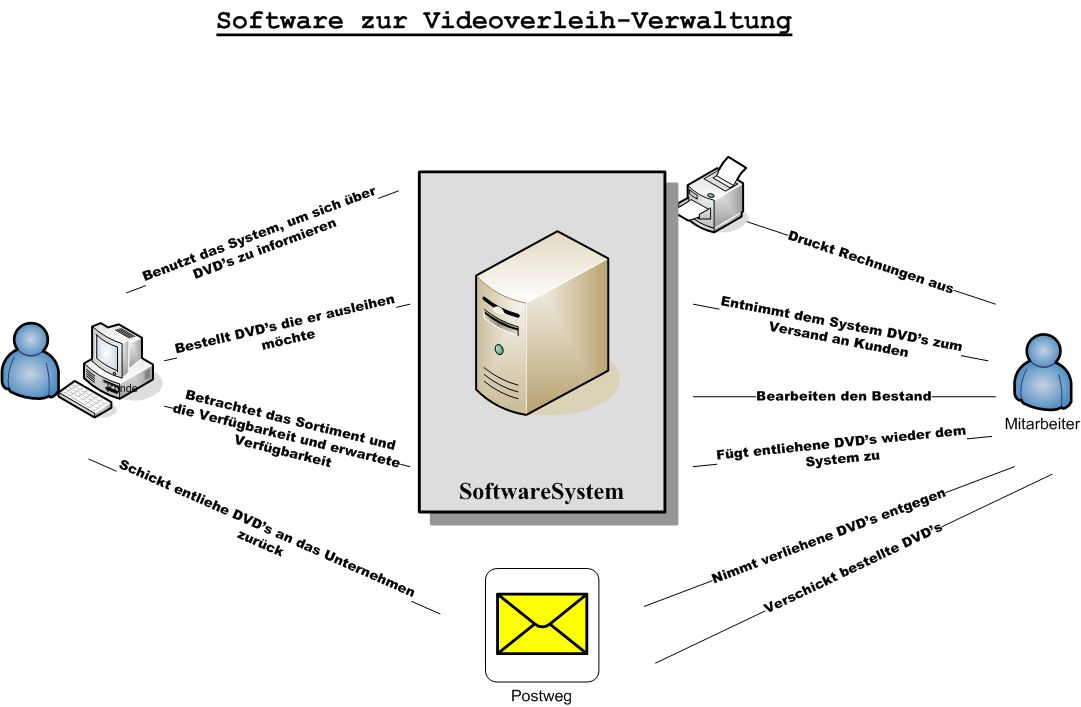
\includegraphics[scale=0.65]{images/erste-gedanken.jpg}
	}
	\caption{Erste Gedanken zu der Videosoftware}
	\label{fig:erstegedanken}
\end{figure}
%===========================================
Nach einiger �berlegung wurde festgestellt, das die Software aus drei anstatt zwei Modulen bestehen muss, wie in \vref{fig:dreimodule} zu sehen ist. Bei den Mitarbeitern der Online-Videothek muss in Verwaltung und Versand/Lagen unterschieden werden, da diese unterschiedlichen Aufgaben von unterschiedlichen Mitarbeitern bearbeitet werden. Das \textbf{Kundenmodul} ist die Internetpr�senz der Videothek und repr�sentiert das Unternehmen nach aussen. Auf dieser dynamischen Webseite kann der Kunde die vorhanden Videos durchst�bern und detaillierte Informationen zu den Videos erhalten. Nach erfolgreicher Anmeldung im System kann der Kunde die Verf�gbarkeit des jeweiligen Videos kontrollieren und auf Wunsch Videos ausleihen. In einem zus�tzlichen Men�punkt kann er seine bestellten Videos betrachten und sich ggf. Rechnungen ausdrucken. Das \textbf{Versandmodul} stellt die ben�tigte Software f�r das Lager und den Versand zur Verf�gung. Mit deren Hilfe kann ein Mitarbeiter der Online-Videothek Videos f�r den Versand vorbereiten. D.h. der Mitarbeiter bekommt eine Liste mit Bestellungen von Kunden (elektronisch oder auf Papier) und arbeitet diese ab. Damit der Mitarbeiter nicht jedes mal die Kundennummer und Nummern der Videos eintippen muss, wird seine Arbeit durch Barcodes und Barcodescanner unterst�tzt. Mit dessen Hilfe markiert er Videos f�r einen bestimmten Kunden und eine bestimmte Bestellung und versendet diese. Dem System teilt der Mitarbeiter dadurch mit, das bestimmte Videos nicht mehr verf�gbar sind und von einem bestimmten Kunden ausgeliehen wurde. Rechnungen, Versandetiketten und eventuelle Lieferscheine werden dabei automatisch mit Hilfe eines Druckers erstellt. Zus�tzlich bietet das Versandmodul die M�glichkeit, zur�ckgekommene Videos der Kunden wieder in das System aufzunehmen. Somit wurde das Video wieder vom Kunden zur�ckgegeben und es kann im System als vorhanden/ausleihbar markiert werden oder gleich an den n�chsten Kunden weitergeschickt werden. Das \textbf{Verwaltungsmodul} hilft den Mitarbeitern in der Verwaltung bei der Organisation der Online-Videothek. Es k�nnen Kundendaten und Rechnungen betrachtet und ggf. gedruckt werden. Das Videosortiment kann bearbeitet und inhaltliche �nderungen (z.B. Sonderangebote) an dem Kundenmodul vorgenommen werden. Weiterhin besteht die M�glichkeit ausf�hrliche Reports \& Statistiken zu erstellen und zu betrachten.\\
%===========================================
\begin{figure}[tbp]
	\centering
	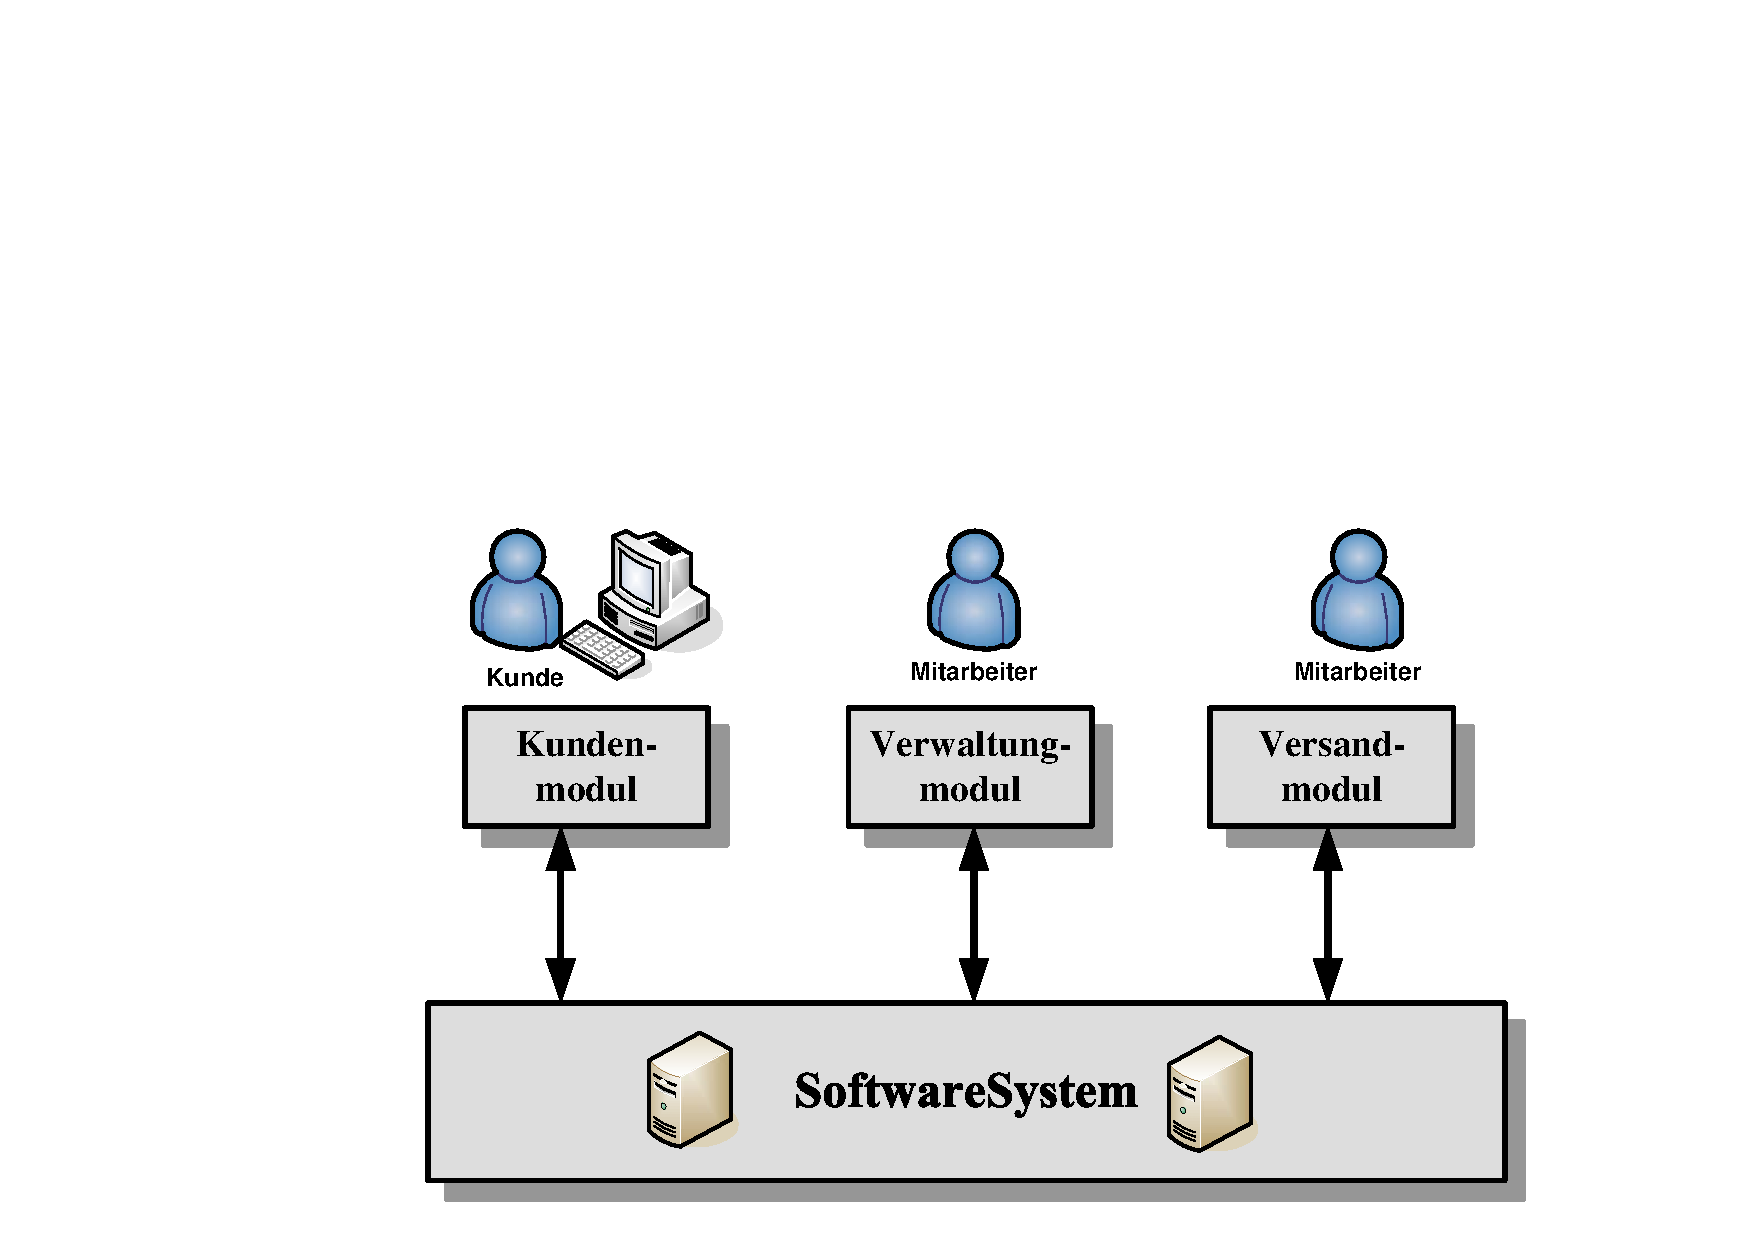
\includegraphics[scale=0.65]{images/dreimodule.pdf}
	\caption{Die drei Module der Software}
	\label{fig:dreimodule}
\end{figure}
%===========================================


%===========================================
\subsection{das Kundenmodul im Detail} \label{sec:Kundenmodul}
Das Kundenmodul ist das wichtigste Element der Anwendung, denn dieses Modul wird vom Kunden verwendet und dieser bestimmt �ber Erfolg oder Misserfolg der Online-Videothek und damit �ber die Anwendung. Das Kundenmodul wird, wie bereits erkl�rt, als Webanwendung entwickelt. Somit muss der Nutzer keine spezielle Software auf seinem Rechner verwenden und kann die Software somit �berall verwenden. Grunds�tzlich wird bei der Anwendung zwischen zwei verschiedenen Kundengruppen unterschieden: dem \emph{Interessenten} und dem \emph{angemeldeten Kunden}. Ein \emph{Interessent} ist ein Websurfer, der sich �ber das Angebot der Online-Videothek interessiert, ohne bisher ein Video ausgeliehen zu haben. Ist der Interessent von dem Angebot �berzeugt und m�chte ein Video ausleihen, muss er sich im System registrieren. Dazu geh�rt neben einem Benutzernamen und Passwort auch seine vollst�ndige Adresse, f�r den Versand der Videos bzw. Rechnungen, und seine Bankverbindung bzw. Kreditkartendaten, f�r die Bezahlung. Ist Kunde in das System eingeloggt, ist er ein angemeldeter Kunde. Je nach Kundengruppe pr�sentiert sich die Webseite mit anderen Funktionalit�ten. Zuerst sollen die Funktionen und M�glichkeiten eines Interessenten erkl�rt werden. Der Interessent hat kann sich auf der Webseite der Online-Videothek sowohl �ber das Angebot an Videos, als auch �ber die Online-Videothek informieren. �ber verschiedene Webseiten erh�lt er Einblick in die f�r ihn interessante Funktionsweise der Online-Videothek und allgemeinen Daten, wie Impressum, Kontaktdaten und Allgemeine Gesch�ftsbedingungen. �ber eine intelligente Suche und Navigationselementen kann er nach Videos suchen bzw. st�bern. Die Videos sind kategorisiert bzw. geordnet. Der Interessent kann auch detaillierte Informationen �ber einzelne Filme erhalten. Dabei kann er sich �ber die Features des Filmes informieren, Kommentare bzw. Bewertungen lesen und �hnliche Filme betrachten. Die dabei verwendete Suche wird als inteligente Suche bezeichnet, weil diese Suche auch �hnliche bzw. verwandte Filme findet und  sowohl im Titel, als auch in der Beschreibung der Filme nach dem Stichwort sucht. Es k�nnte auch realisiert werden, das die Suchergebnisse nach Trefferquoten geordnet werden bzw. das Suchfeld automatisch das Wort nach h�ufigen Suchbegriffen erg�nzt.\\
Ist der User eingeloggt hat er die gleiche Funktionsweise wie ein Interessent, nur mit erweiterten Funktionen. In der Ergebnissliste der Suche oder der Anzeigeliste der Kategorien, welche beide gleich aufgebaut sind, befinden sind neben jedem Video Elemente zum bestellen und zum �berpr�fen der Verf�gbarkeit. Jedes Video, also jeder Film, ist in einer gewissen Anzahl vorhanden. Mit Hilfe der �berpr�fung der Verf�gbarkeit kann der Kunde �berpr�fen, ob noch ein Video dieses Filmes f�r ihn zum Ausleihen vorhanden ist, bzw. wann das n�chste Video wieder verf�gbar ist. Je nach Status der Verf�gbarkeit kann der Kunde das Video in seinem Warenkorb legen und damit ausleihen, oder vormerken lassen. Bei einer Vormerkung wird er entweder per Email informiert, dass das Video vorhanden ist, oder das Video wird schnellstm�glich an den Kunden versendet. Hat der Kunden Videos in seinen Warenkorb abgelegt, kann dieser am Ende seiner Bestellung zur Kasse gehen und somit die Videos ausleihen. Weiterhin hat der Kunde die M�glichkeit eine so genannte \emph{Wunschliste} zu Erstellen. Diese Liste kann eine bestimmte Anzahl an Videos anschauen, die der Kunde schauen m�chte. Das System arbeitet diese Liste automatisch ab, indem es dem Kunden eine bestimmte Anzahl an Videos mit einmal zusendet und bei R�cksendung durch den Kunden die n�chsten Filme automatisch an den Kunden sendet. Somit hat der Kunden z.B. die M�glichkeit 50 Filme zu bestimmen, die er gerne anschauen m�chte. Das System sendet ihm immer zwei Filme mit einmal zu, die er sich anschauen kann. Sendet er diese zwei Filme zur�ck, bekommt er die n�chsten zwei Filme, bis die Liste abgearbeitet wurde. Weiterhin bietet das Kundenmodul dem Kunden die M�glichkeiten, �ltere und aktuelle Bestellungen bzw. Vorbestellungen zu betrachten, Rechnungen auszudrucken und allgemeine Einstellungen an seinem Profil vorzunehmen. Das Kundenmodul soll dabei einfach und ohne Bedienungsanleitung zu bedienen sein, der Kunden soll sich schnell zu recht finden und schnell zu seinem Ziel, einer Bestellung, kommen.\\


%===========================================
\subsection{das Versandmodul im Detail} \label{sec:Versandmodul}
Das Versandmodul ist der Bestandteil der Videothek in der die Arbeit geschieht. Hier werden Videos herrausgesucht, verpackt und an den Kunden versendet. Dabei wird der Mitarbeiter soweit wie M�glich von der Technik unterst�tzt. Bei dieser Technik handelt es sich haupts�chlich um Barcodescanner. Ein Barcodescanner ist ein Leseger�t, das mit Hilfe eines Lasers einen Strichcode auf einer Verpackung oder einem Blatt liest. Dieser Strichcode kann dabei je nach Art und Weise eine Nummer oder einen Wort repr�sentieren. Diese Strichcodes sind aus dem heutigen Alltag nicht wegzudenken, denn sie sind auf jeder Verpackung vorhanden und werden in Superm�rkten als Preisschild verwendet. Dabei hat jedes Produkt eine eindeutige Nummer, zu der mit Hilfe einer Datenbank ein Preis zugeordnet wird. Neben Strichcodes gibt es noch zweidimensionale Codes, die mehr Informationen speichern k�nnen.\\
%%http://www.4mation.com.au/images/softwaredevelopment/products/softwaredevelopment_barcodescanner.jpg
%%http://jbars.sourceforge.net/
%%http://jbarcodebean.sourceforge.net/
\begin{figure}[htbp]
	\centering
	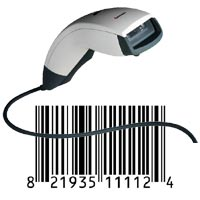
\includegraphics[scale=1.0]{images/Barcodescanner.jpg}
	\caption{Abbildung eines Barcodescanners}
	\label{fig:barcodescanner}
\end{figure}
An einem Zentralen Rechner werden die Bestellungen der Kunden ausgedruckt. Solch ein Ausdruck besteht aus einer Seite, auf der oben zwei Adressetiketten und unten einem Lieferschein vorhanden sind. Das erste Adressetikett ist das f�r den Versand zu dem Kunden, das auf den Umschlag der Bestellung geklebt wird. Das zweite ist dasjenige, welches der Kunde auf dem Umschlag zur R�cksendung der Video klebt. Der Lieferschein ist sowohl f�r den Mitarbeiter als auch f�r den Kunden wichtig. Der Mitarbeiter liest mit Hilfe eines Barcodescanners die Bestellnummer ein. Aus dieser Rechnungsnummer kann der Computer sowohl auf den Kunden als auch auf die Videos schlie�en, die versendet werden sollen. Der Mitarbeiter sucht, mit Hilfe einer weiteren Software den Lagerort der jeweiligen Videos heraus und scannt deren eindeutige Nummer. Damit sind die Videos im System nicht mehr verf�gbar und dem Kunden zugeordnet. Anschlie�end verpackt er die Videos in einen entsprechenden Umschlag und verschickt die Videos mit dem Ausdruck an dem Kunden. Bei diesem Vorgang gibt es mehrere M�glichkeiten wie der Mitarbeiter vorgehen kann. Damit der Mitarbeiter nicht f�r jede Bestellung durch das Lager gehen muss, kann das System eine Liste mit Videos erstellen, f�r die n�chsten 10 Bestellungen. Somit sucht der Mitarbeiter diese Videos heraus und bearbeitet nacheinander diese zehn Bestellungen. Eine weitere M�glichkeit w�re, das der Mitarbeiter und das Lager durch ein automatisiertes Lager ersetzt wird. Dabei �bernimmt ein Roboter in einem Lager die Aufgabe des Suchen und Finden der Videos. Schickt der Kunde die Videos an die Online-Videothek zur�ck, nimmt ein Mitarbeiter die Videos entgegen. Zuerst scannt er dabei die Bestellnummer und die eindeutige Nummer des jeweiligen Videos. Zus�tzlich muss er den Zustand der Videos �berpr�fen und im System eintragen. Anschlie�end sind die Videos wieder im System verf�gbar und k�nnen wieder eingeordnet werden oder an den n�chsten Kunden versendet werden.\\
Das komplette Lager k�nnte durch spezielle Maschinen vollst�ndig automatisiert werden. Diese Maschinen w�rden dann automatisch das Suchen und das Verpacken der Videos �bernehmen. Dabei w�rden wieder Barcodescanner zum Einsatz kommen, um die Bestellnummern und Videonummers automatisch einzulesen. Solch ein System w�rde sich aber nur bei einer sehr grosser Online-Videothek rentieren, da der Anschaffungspreis solcher Maschinen enorm ist.

\begin{figure}[tbp]
	\centering
	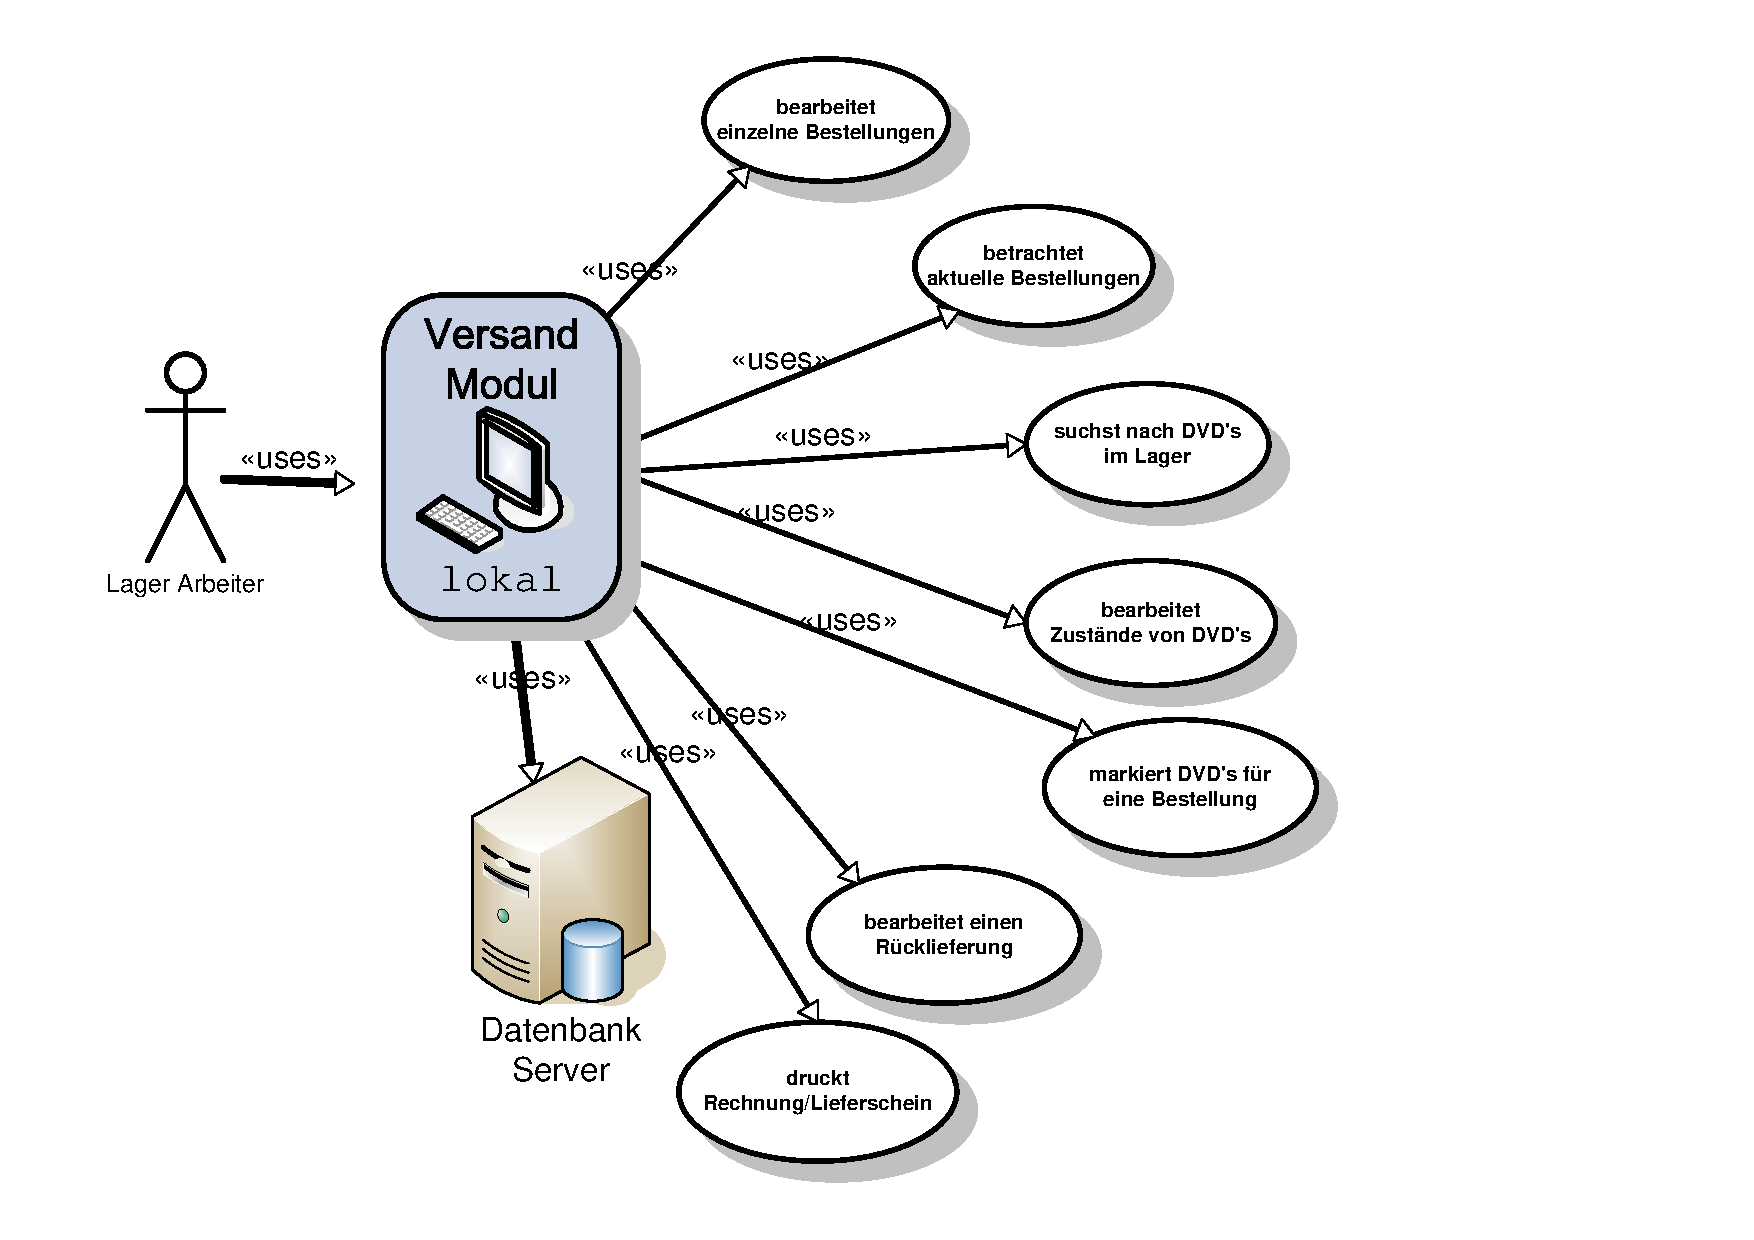
\includegraphics[scale=1.0]{images/usecase-versandmodul.pdf}
	\caption{UseCase Versandmodul}
	\label{fig:usecaseversand}
\end{figure}
	 	
%===========================================
\subsection{das Verwaltungsmodul im Detail}  \label{sec:Verwaltungsmodul}
Das Verwaltungsmodul ist f�r die Verwaltung der Online-Videothek in B�ror�umen gedacht. Die Mitarbeiter des Unternehmens haben dabei Einblick in die verschiedenen Daten der Online-Videothek und k�nnen diese, sollten sie die ben�tigten Rechte besitzen, ver�ndern. Unter zu Hilfenahme des Verwaltungsmodul k�nnen neue Videos in System aufgenommen werden. Dazu wird zuerst der jeweilige Film hinzugef�gt und danach die einzelnen Videos dieses Filmes. Dabei werden sich wiederholende Daten wie Darsteller oder Genre in eigenen Elementen gespeichert. Nachdem der Mitarbeiter mit dem Hinzuf�gen von neuen  Videos fertig ist, werden diese automatisch im Kundenmodul verf�gbar sein. Mit Hilfe dieses Moduls k�nnen auch Kundendaten betrachtet oder ver�ndert werden. Somit kann z.B. eine Telefonhotline oder der Kundensupport Fragen der Kunden zu einzelnen Bestellungen beantworten. F�r die Gesch�ftsleitung k�nnen ausf�hrliche Statistiken erstellt werden.\\
Das Verwaltungsmodul stellt somit ...
\begin{figure}[htbp]
	\centering
	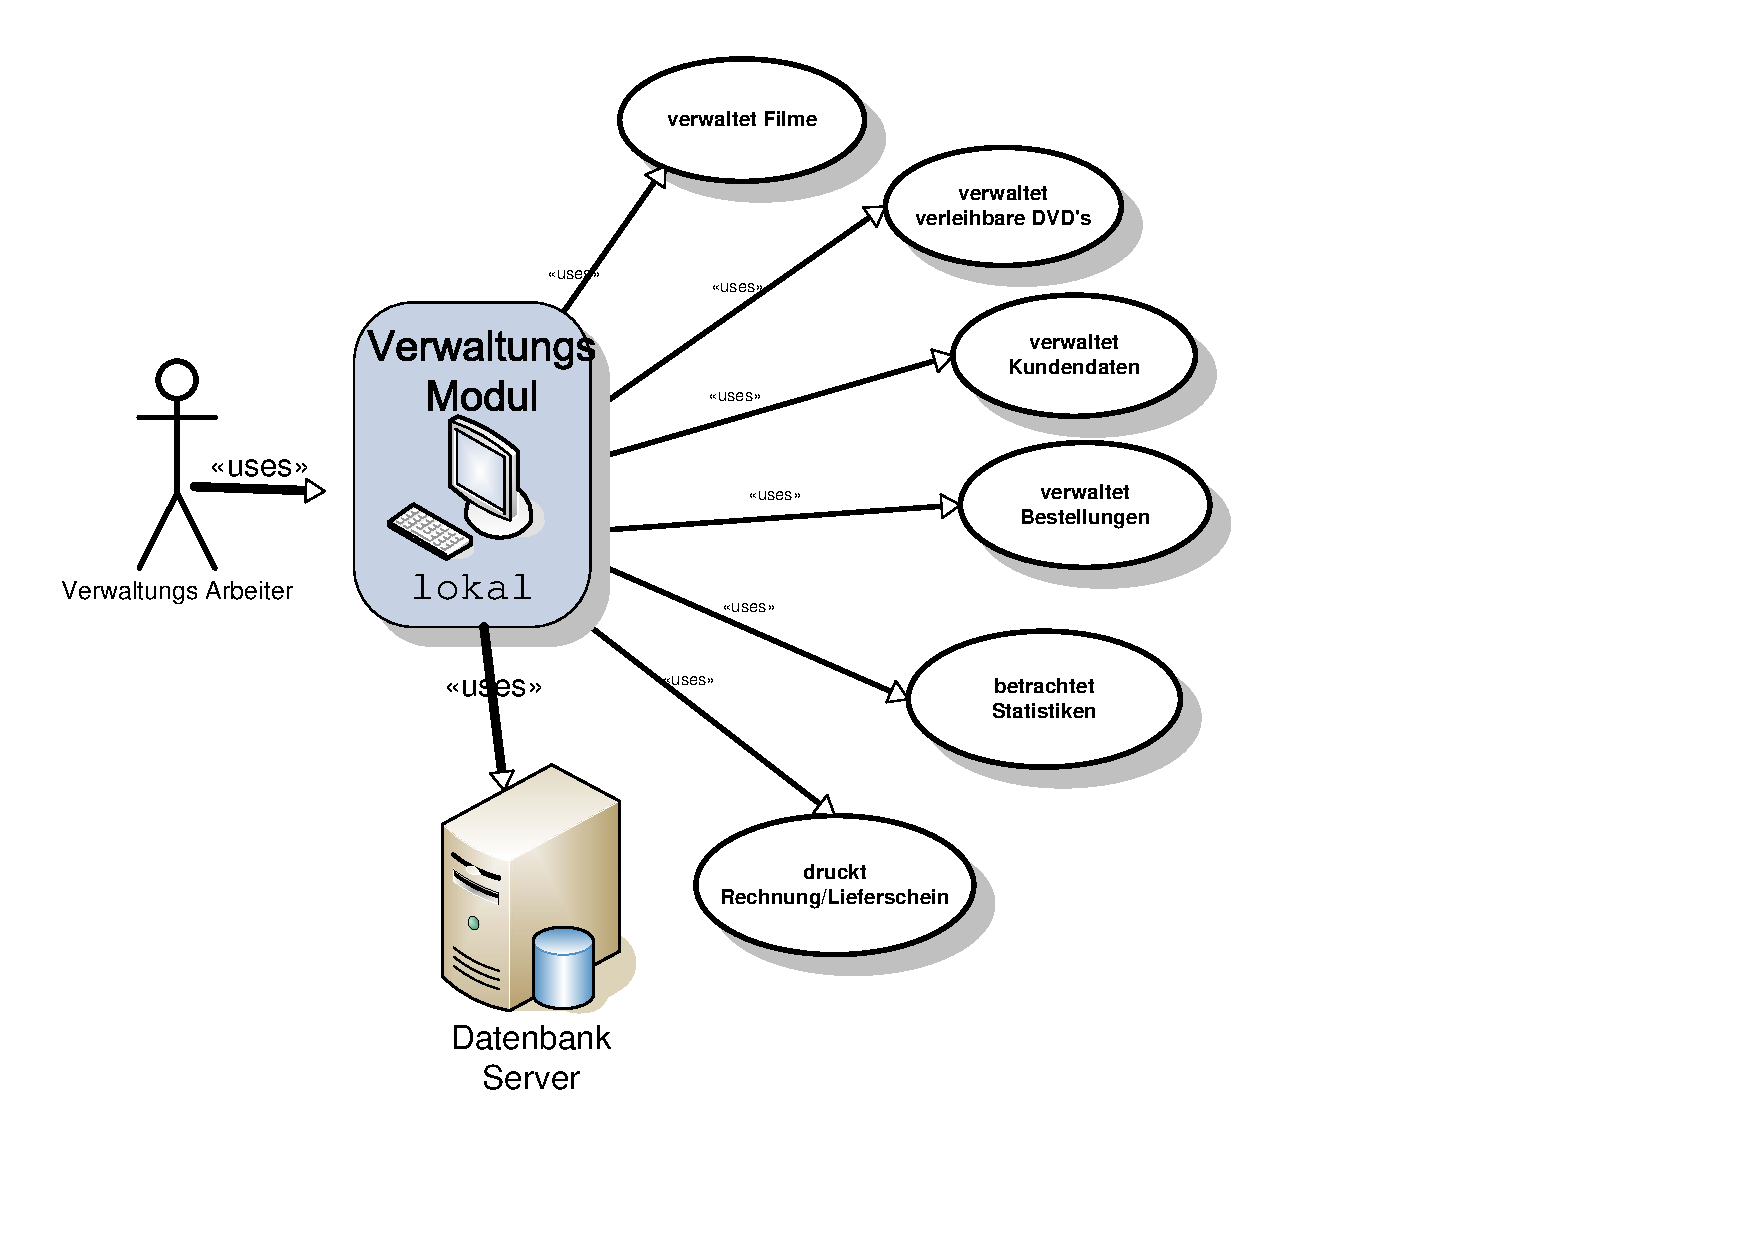
\includegraphics[scale=1.0]{images/usecase-verwaltungsmodul.pdf}
	\caption{UseCase Verwaltungsmodul}
	\label{fig:usecaseverwaltung}
\end{figure}



%===========================================
\section{geplante Module und Versionen}
Da dieses Projekt nach ersten �berlegungen und Planungen nicht nur ein kleiner Projekt ist, wurde beschlossen, zuerst das Verwaltungsmodul, dann das Kundenmodul und danach das Versandmodul zu implementieren. Das Verwaltungsmodul ist das Herzst�ck der Online-Videothek. Hier werden die Daten erstellt und verwaltet, die von den beiden anderen Modulen verwendet werden. Das Verwaltungsmodul und das Versandmodul, soll dabei eine Anwendung auf einem beliebigen Rechner innerhalb des Firmennetzwerks sein. Das Kundenmodul hingegen soll eine weltweit verwendbare Webanwendung sein. Mit der Realisierung des Verwaltungsmodul wurde zuerst begonnen.\\


Das Kundenmodul und das Versandmodul konnten aus Zeitgr�nden nicht mehr realisiert werden.\\


\chapter{Technologien} \label{sec:Technologien}
In diesem Abschnitt werden kurz die zu verwendeten Technologien verwendet.

	
\section{Datenbank}
Zum Einsatz soll eine OpenSource Datenbank kommen. Gedanken an eine kommerzielle Datenbank kam aus Gr�nden der Lizenzkosten nicht auf. \\
Zu Auswahl standen mehrere OpenSource Datenbanken. MySql \footnote{\url{http://dev.mysql.com/downloads/mysql/4.0.html}}, SAP DB \footnote{\url{http://dev.mysql.com/downloads/maxdb/7.5.00.html}} , HSQL DB \footnote{\url{http://hsqldb.sourceforge.net}} und Firebird \footnote{\url{http://firebird.sourceforge.net}}.
		\begin{itemize}
			\item \textbf{MySql}
				\begin{itemize}
					\renewcommand{\labelitemii}{+}
					\item sehr verbreitet
					\item einige Erfahrung
					\item gut Dokumentiert \& gro�e Community
					\item 
				\end{itemize}
				
				\begin{itemize}
					\item schlechtes Lizenzmodell
					\item zu bekannt
					\item keine Trigger
					\item meist nur im privat bzw. klein Unternehmer Einsatz
				\end{itemize}
				
			\item \textbf{SAP DB}
				\begin{itemize}
					\renewcommand{\labelitemii}{+}				
					\item 
					\item Datenbank seit mehreren Jahren bei SAP im Einsatz
				\end{itemize}
				
				\begin{itemize}
					\item schlechte Skalierbarkeit, da der Datenbank Speicherbereich im Vorfeld festgelegt werden muss
					\item schlechte Erfahrung
				\end{itemize}
				
			\item \textbf{HSQLDB}
				\begin{itemize}
					\renewcommand{\labelitemii}{+}				
					\item reine JavaDatenbank
					\item sehr klein
					\item kann als reine Speicher Datenbank verwendet werden (Daten nur im Arbeitsspeicher)
					\item kann als Applikations Datenbank verwendet werden (nur eine Applikation benutzt die Datenbank)
				\end{itemize}
				
				\begin{itemize}
					\item nicht f�r gro�e Applikationen geeignet
					\item 
				\end{itemize}			

			\item \textbf{Firebird}
				\begin{itemize}
					\renewcommand{\labelitemii}{+}				
					\item geringe Erfahrung durch Studium
					\item sehr klein
					\item gute grafische Tools
					\item Original Sourcen kommen von Borland
					\item Interbase Datenbank seit mehreren Jahren im Professionelle einsatz
				\end{itemize}
				
				\begin{itemize}
					\item schlechtes Lizenzmodell
					\item 
				\end{itemize}
		
		\end{itemize}
		
Wir haben uns f�r die Firebird Datenbank entschieden, da es keine wirkliche Konkurrenz im Open Source Bereich gibt.\\
HSQL scheidet schon aus, weil es nicht f�r grosse Datenmengen geeignet ist. Bei der SAP DB muss der ben�tigte Speicherplatz der Datenbank vorher bekannt sein, was bei unserem Projekt nicht der Fall ist. MYSQL unterst�tzt keine Triggers und ist zu bekannt, d.h. MySql kann und sollte jeder Informatiker kennen und benutzt haben. \\
Firebird ist f�r uns relativ neu und die Erfahrungen die wir in der Vorlesung "`Datenmanagment 2"' bekommen haben, war sehr positiv. Da diese Datenbank urspr�nglich von Borland kommt, ist diese Datenbank auch nicht so neu, wie viele Denken.\\
Es soll aber schon am Anfang des Projektes bedacht werden, dass die Datenbank zu einem sp�teren Zeitpunkt eventuell mit einer professionelle Datenbank\footnote{z.B. DB2 von IBM} ausgetauscht werden k�nnte. Deswegen muss schon am Anfang eine hohe Abstraktionsebene vorhanden sein, so dass eventuelle Datenbankspezifische Elemente (Klassen) sehr einfach ausgetauscht werden k�nnen.
		
		
				
\section{Versionsverwaltung}
Eine Versionsverwaltung 


\url{http://better-scm.berlios.de/comparison/comparison.html}
\citep[Versionsverwaltung]{Wikipedia2005}

		\subsection{Concurrent Versions System - CVS}
		\subsection{Subversion}
		
\section{Entwicklungsumgebung}
		\subsection{JBuilder}
		\subsection{Netbeans}
		\subsection{Eclipse}

\section{grafischen Benutzerschnittstellen in Java}
		\subsection{Abstract Window Toolkit - AWT}
		\subsection{Swing}
		\subsection{Standard Widget Toolkit - SWT}
		
\section{Java-Web-Anwendungen}
		\subsection{Java Server Faces - JSF}
		\subsection{Struts}

\section{Persistenzschichten in Java}
		\subsection{Java Data Objects}
		\subsection{Hibernate}
		
		
		
		

		
\section*{Datenbank - erste Ideen}	\label{asas}




	\begin{itemize}
			
  		\item Kunden
  		\begin{itemize}
  			\setlength{\itemsep}{-1ex plus0.5ex minus0.3ex}
  			\item kundenid \emph{Integer Autoincrement Primary Key}
  			\item name \emph{VARCHAR(200)}
  			\item vorname \emph{VARCHAR(200)}
  			\item strasse \emph{VARCHAR(200)}
  		\end{itemize}
  	 \item benutzer
  		\begin{itemize}
  			\setlength{\itemsep}{-1ex plus0.5ex minus0.3ex}
  			\item benutzerid \emph{Integer Autoincrement Primary Key}
  		\end{itemize}

  	 \item dvds
  		\begin{itemize}
  			\setlength{\itemsep}{-1ex plus0.5ex minus0.3ex}
  			\item dvdid \emph{Integer Autoincrement Primary Key}
  		\end{itemize}

  	 \item genre
  		\begin{itemize}
  			\setlength{\itemsep}{-1ex plus0.5ex minus0.3ex}
  			\item genreid \emph{Integer Autoincrement Primary Key}
  		\end{itemize}

  	 \item artikel
  		\begin{itemize}
  			\setlength{\itemsep}{-1ex plus0.5ex minus0.3ex}
  			\item artikelid \emph{Integer Autoincrement Primary Key}
  		\end{itemize}

  	 \item verleih
  		\begin{itemize}
  			\setlength{\itemsep}{-1ex plus0.5ex minus0.3ex}
  			\item verleihid \emph{Integer Autoincrement Primary Key}
  		\end{itemize}

  	 \item preis
  		\begin{itemize}
  			\setlength{\itemsep}{-1ex plus0.5ex minus0.3ex}
  			\item preisid \emph{Integer Autoincrement Primary Key}
  		\end{itemize}
  	 

   \end{itemize}			

	\section*{Prototyp}
	Bevor versuchen ein fertiges Produkt zu realisieren und daran vermutlich scheitern werden, haben wir beschlossen einen einfachen Prototyp zu programmieren. Dieser soll die wichtigsten Merkmale besitzen und zu Demostrationszwecken dienen.
	Jedoch soll es auch m�glich sein, diesen Prototypen zu einem fertigen Produkt fertig zu entwickeln. Der Prototyp soll also nicht quick \& dirty programmiert werden. \\
	Der Prototyp soll haupts�chlich die Kundenseite implementieren. D.h. er soll eine Webanwendung bereitstellen, bei der der Kunde bzw. Interessent sich regiestrieren kann und die Videothek benutzen kann. Dies bedeutet er kann sich die vorhanden Videos anschauen (Informationen zu diesen), kann sich die Verf�gbarkeit anschauen, Video ausleihen, Rechnungen ansehen bzw. ausdrucken und eine Liste mit all seinen bisherigen Bestellungen anschauen. \\
	Das Modul f�r die Verwaltung der DVD's ist in diesem Prototypen noch nicht vorgesehen. \\
	Das Modul f�r das Versenden und Empfangen ist nur in einfacher Variante vorgesehen. Der Mitarbeiter der Onlinevideothek bekommt eine kleine Anwendung auf Konsolenbasis ohne grafische Oberfl�che.
		
		
\chapter{Implementierung} \label{sec:Implementierung}

\section{Versionsverwaltung mit Subversion}
\footnote{So wird eine Fussnote gemacht}\\
% das ist ein Kommentar
\url{http:/www.phil-schneider.de}
\citep{Frotscher2004b} Verweis auf eine Literaturquelle
\emph{hervorgehoben}\\
\textbf{Fett}\\
\texttt{Typewriter}\\

		
\section{Entwicklungsumgebung mit Eclipse}

\section{grafischen Benutzerschnittstellen mit SWT}
		
\section{Java-Web-Anwendungen mit Struts}


\section{Persistenzschichten mit Hibernate}
\chapter{Zusammenfassung} \label{sec:Zusamenfassung}


\appendix
\chapter{Protokoll vom 11. Mai 2004}

Drei Frameworks stehen zur Auswahl \\
\begin{itemize}
	\item Apache Cocoon
	\item Apache Struts
	\item Apache Tapestry
\end{itemize}

Jeder erstellt eine einfache (Web)Anwendung mit Hilfe eines dieser Frameworks 
folgende Komponenten sollen/muessen enthalten sein: \\
\begin{itemize}
	\item einfache LoginSeite (�ber Datenbank)
	\item Liste aller Videos in Datenbank anzeigen
	\item EingabeMaske f�r neues Labor
	\item Validierung der Eingabedaten
	\item dynamische Navigation
	\item eventuell ein Bild f�r den Status der einzelnen Bilder (dynamisches Bild??)
\end{itemize}

F�r diese BeispielAnwendung sollen m�glichst viele Elemente des jeweiligen Framework verwendet werden.
Wichtig ist dabei der Umgang und die Bedienbarkeit des Systems. \\
Wiederverwendbarkeit einzelner Module. \\
Design und Logik Trennung vorhanden? Kann das Design einfach/schnell ausgetauscht werden.\\
\\
Es geht dabei nicht um ein 100% fehlerfreies System.\\
Design spielt keine wichtige Rolle, es sollte jedoch beachtet werden, dass dieses sp�ter vom Kunden ausgetauscht werden m�chte.\\
\\
\\
\begin{itemize}
	\item Struts: Stefan
	\item Cocoon: Philipp
	\item Tapestry: Remo
\\
	\item Namen f�r das Projekt finden
	\item Link mit Beispiel Webseiten rumschicken
\end{itemize}
	
%%%%%%%%%%%%%%%%%%%%%%%%%%%%%%%%%%%%%%%%%%%%%%%%%%%%%%%%%%%%%%%%%
% 																															%
%---------------------------------------------------------------%
%                         9-1Literatur.tex                      %
%%%%%%%%%%%%%%%%%%%%%%%%%%%%%%%%%%%%%%%%%%%%%%%%%%%%%%%%%%%%%%%%%

%\nocite{Wessel2005}
\addcontentsline{toc}{chapter}{Literaturverzeichnis}
\bibliography{Provirent-Doku}
%%%%%%%%%%%%%%%%%%%%%%%%%%%%%%%%%%%%%%%%%%%%%%%%%%%%%%%%%%%%%%%%%%
% 																															%
%---------------------------------------------------------------%
%            9-2Abkuerzungsverzeichnis.tex                      %
% Abk�rzungen sp�ter in den Text direkt uebernehmen, dort wie diese das erste mal verwendet werden, somit 
% kann mittels refpage auf die Seite verwiesen werden
%%%%%%%%%%%%%%%%%%%%%%%%%%%%%%%%%%%%%%%%%%%%%%%%%%%%%%%%%%%%%%%%%
\addcontentsline{toc}{chapter}{Abk�rzungsverzeichnis}


\printnomenclature
%\addcontentsline{toc}{chapter}{Index}
%\printindex
%%%%%%%%%%%%%%%%%%%%%%%%%%%%%%%%%%%%%%%%%%%%%%%%%%%%%%%%%%%%%%%%%%
% 																															%
%---------------------------------------------------------------%
%                        9-2Erklaerung.tex                      %
%%%%%%%%%%%%%%%%%%%%%%%%%%%%%%%%%%%%%%%%%%%%%%%%%%%%%%%%%%%%%%%%%
\addcontentsline{toc}{chapter}{Erkl�rung}
\chapter*{Erkl�rung}

\vspace*{2cm}
Ich erkl�re hiermit, dass ich zur Anfertigung der vorliegenden Arbeit keine anderen als die angegebenen Quellen und Hilfsmittel und keine nichtgenannte fremde Hilfe in Anspruch genommen habe. Mir ist bewusst, dass eine falsche Versicherung rechtliche Konsequenzen hat.

\vspace{4cm} Leipzig, den \today  \\





%------ Ende des Dokumentes ------
\end{document}